% Prof. Dr. Ausberto S. Castro Vera
% UENF - CCT - LCMAT - Curso de Ci\^{e}ncia da Computa\c{c}\~{a}o
% Campos, RJ,  2023
% Disciplina: An\'{a}lise e Projeto de Sistemas
% Aluno: 
 

\chapterimage{conclusoes.png} % Table of contents heading image
\chapter{Considera\c{c}\~{o}es Finais} 


Esse trabalho abordou a modelagem de um sistema já utilizado e conhecido: o monitoramento de entregas em tempo real, que representa um avanço significativo na otimização e eficiência das operações logísticas. Ao longo deste trabalho, identificamos e abordamos diversos desafios enfrentados durante o desenvolvimento e implementação do sistema. Estes desafios incluíram questões relacionadas à integração de diferentes tecnologias e a falta de conhecimento de como se dá o funcionamento desses tipos de sistemas a nível de mercado.

O sistema de monitoramento em tempo real pode demonstrar ser uma ferramenta crucial para aprimorar a eficiência operacional, reduzir custos e melhorar a satisfação do cliente. A capacidade de rastrear e visualizar as entregas em tempo real não apenas proporcionou maior transparência, mas também possibilitou a antecipação e solução proativa de possíveis problemas, como atrasos ou desvios.

Diante desse contexto, fica evidente que a modelagem de sistemas de monitoramento de entregas em tempo real é uma estratégia vital para empresas que buscam se destacar em um ambiente logístico dinâmico e desafiador.


   \begin{figure}[H]
    \begin{center}
        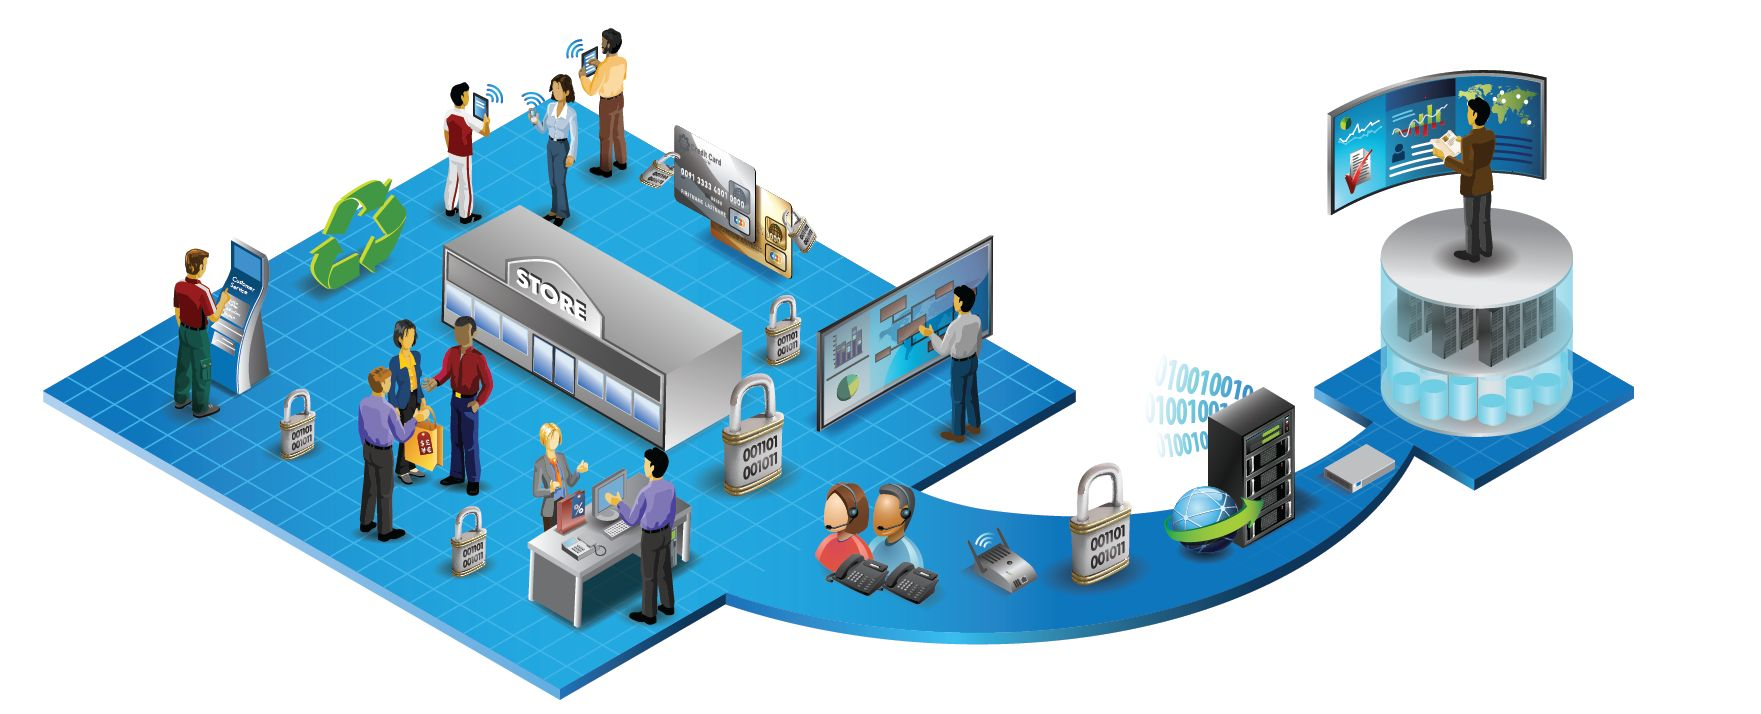
\includegraphics[width=12cm]{MeuSistema.jpg}
        \caption{Meu Sistema a ser desenvolvido} \label{sistema}
    \end{center}
   \end{figure} 